\documentclass[aspectratio=169]{beamer}

\usepackage{Archivo}
\renewcommand{\sfdefault}{\rmdefault}
\usepackage{graphicx}
\usepackage{tikz}
\usetikzlibrary{calc,positioning}
\tikzset{
  invisible/.style={opacity=0, text opacity=0},
  visible on/.style={alt={#1{}{invisible}}},
  alt/.code args={<#1>#2#3}{%
    \alt<#1>{\pgfkeysalso{#2}}{\pgfkeysalso{#3}}%
  },
}
\usepackage[most]{tcolorbox}
\usepackage{listings}

%% ---- Superteam Poland brand colors ----
\definecolor{stpldark}{HTML}{0B0E0F}   % near-black background
\definecolor{stplcard}{HTML}{161A1B}   % card / block surface
\definecolor{stplborder}{HTML}{1E2526}  % subtle track color for progress bar
\definecolor{stplred}{HTML}{DC143C}    % brand crimson red
\definecolor{stplwhite}{HTML}{FFFFFF}  % white
\definecolor{stplmuted}{HTML}{8A9BA8}  % muted / secondary text

\usetheme{default}
\setbeamersize{text margin left=0.85cm, text margin right=0.85cm}

%% ---- Background & base text ----
\setbeamercolor{background canvas}{bg=stpldark}
\setbeamercolor{normal text}{fg=stplwhite, bg=stpldark}
\usebeamercolor{normal text}

%% ---- Background image helpers ----
\newcommand{\stpldefaultbg}{%
  \setbeamertemplate{background}{%
    \begin{tikzpicture}[remember picture, overlay]
      \node[at=(current page.center), inner sep=0pt] {%
        \includegraphics[width=\paperwidth,height=\paperheight]{images/bg-default.png}%
      };
      \fill[stplborder]
        (current page.north west) rectangle
        ([yshift=-2.5pt]current page.north east);
      \pgfmathsetmacro{\stplprog}{\insertframenumber/\inserttotalframenumber}
      \fill[stplred]
        (current page.north west) rectangle
        ($(current page.north west)+(\stplprog\paperwidth,-2.5pt)$);
    \end{tikzpicture}%
  }%
}
\newcommand{\stplherobg}{%
  \setbeamertemplate{background}{%
    \includegraphics[width=\paperwidth,height=\paperheight]{images/bg-hero.png}%
  }%
}
\stpldefaultbg

%% ---- Structure ----
\setbeamercolor{structure}{fg=stplred}

%% ---- Title slide metadata ----
\setbeamercolor{title}{fg=stplwhite}
\setbeamercolor{subtitle}{fg=stplred}
\setbeamercolor{author}{fg=stplwhite}
\setbeamercolor{institute}{fg=stplmuted}
\setbeamercolor{date}{fg=stplmuted}

%% ---- Frame title: flat, no box background ----
\setbeamercolor{frametitle}{fg=stplwhite, bg=}
\setbeamerfont{frametitle}{size=\large, series=\bfseries}
\setbeamertemplate{frametitle}{%
  \vspace{0.35cm}%
  {\centering\insertframetitle\par}%
  \nointerlineskip\vspace{0.18cm}%
  \hfil{\color{stplred}\rule{2.2cm}{1.5pt}}\hfil\par%
}



%% ---- Incremental reveals ----
%% Bullets reveal one at a time by default. See style.md §4.5 for the two
%% per-frame opt-outs (static frame: `\begin{frame}<1>{...}`; manually
%% choreographed frame: `\beamerdefaultoverlayspecification{}` at frame top).
\beamerdefaultoverlayspecification{<+->}

%% ---- Bullet items ----
\setbeamercolor{itemize item}{fg=stplred}
\setbeamercolor{itemize subitem}{fg=stplmuted}
\setbeamercolor{itemize subsubitem}{fg=stplmuted}
\setbeamertemplate{itemize item}{\bfseries\textendash}
\setbeamertemplate{itemize subitem}{\small\textendash}
\setbeamercolor{enumerate item}{fg=stplred}
\setbeamercolor{enumerate subitem}{fg=stplmuted}
\setbeamertemplate{enumerate item}{\textcolor{stplred}{\bfseries\insertenumlabel.}}
\setbeamertemplate{enumerate subitem}{\textcolor{stplmuted}{\small\insertenumlabel.}}

%% ---- Blocks (flat left-accent via tcolorbox) ----
\tcbset{
  stplbase/.style={
    enhanced, breakable,
    colback=stplcard, coltext=stplwhite,
    coltitle=stplwhite, fonttitle=\bfseries,
    boxrule=0pt, leftrule=3pt,
    arc=0pt, outer arc=0pt,
    top=5pt, bottom=5pt, left=7pt, right=7pt,
    toptitle=4pt, bottomtitle=4pt,
    titlerule=0pt,
  },
}
\renewenvironment{block}[1]{%
  \pause%
  \begin{tcolorbox}[stplbase, colframe=stplred, title={#1}]%
}{%
  \end{tcolorbox}%
}
\renewenvironment{alertblock}[1]{%
  \pause%
  \begin{tcolorbox}[stplbase, colframe=stplred!75!black,
    colback=stplred!10!stplcard, title={#1}]%
}{%
  \end{tcolorbox}%
}
\renewenvironment{exampleblock}[1]{%
  \pause%
  \begin{tcolorbox}[stplbase, colframe=stplmuted, title={#1}]%
}{%
  \end{tcolorbox}%
}

%% ---- Code listings (Rust + Anchor) ----
\lstdefinelanguage{Rust}{
  keywords={fn,pub,struct,impl,trait,let,mut,self,Self,match,return,for,in,
            if,else,enum,use,mod,as,where,Option,Result,Some,None,Ok,Err,
            u8,u16,u32,u64,i64,u128,bool,String,Vec,Pubkey,Context,msg,vec,
            Account,Signer,Program,System,has_one,init,payer,space,seeds,bump},
  morecomment=[l]{//},
  morestring=[b]",
  sensitive=true,
}
\lstset{
  basicstyle=\ttfamily\scriptsize\color{stplwhite},
  backgroundcolor=\color{stplcard},
  keywordstyle=\color{stplred}\bfseries,
  commentstyle=\color{stplmuted},
  stringstyle=\color{stplmuted},
  showstringspaces=false,
  keepspaces=true,
  columns=fixed,
  basewidth=0.46em,
  frame=leftline,
  framerule=2pt,
  rulecolor=\color{stplred},
  xleftmargin=0.6em,
  aboveskip=0.4em,
  belowskip=0.2em,
  language=Rust,
  escapeinside={(*@}{@*)},
}

%% ---- Code reveal card (line-synced to bullets) ----
%% A block-styled card WITHOUT the block's auto-\pause, so it is visible from
%% the current overlay and its code lines can reveal in step with the itemize
%% bullets via (*@\onslide<k->@*) markers. The listing drops its own
%% background/frame (style=reveal) so the solid card shows through instead of
%% the per-line background going ragged as lines are covered.
\newtcolorbox{codeblock}[1]{stplbase, colframe=stplred, title={#1}}
\lstdefinestyle{reveal}{backgroundcolor={}, frame=none, xleftmargin=0pt,
  aboveskip=0pt, belowskip=0pt}

%% ---- Table of contents ----
\setbeamercolor{section in toc}{fg=stplwhite}
\setbeamercolor{subsection in toc}{fg=stplmuted}
\setbeamertemplate{section in toc}{%
  {\color{stplred}\textbf{\textendash}}\hspace{0.5em}\inserttocsection%
}

%% ---- Footline: minimal ----
%% Transparent bg so the background image shows through (normal text has
%% bg=stpldark, which would paint a flat band over the image's bottom glow).
\setbeamercolor{footline}{fg=stplwhite, bg=}
\setbeamertemplate{footline}{%
  \begin{beamercolorbox}[wd=\paperwidth, ht=0pt, dp=0.55cm]{footline}%
    \hspace{0.85cm}%
    \raisebox{-0.42cm}{\includegraphics[height=0.42cm]{images/stpl-logo.png}}%
    \hfill%
    \raisebox{-0.24cm}{\textcolor{stplmuted}{\tiny\insertframenumber\,/\,\inserttotalframenumber}}%
    \hspace{0.85cm}%
  \end{beamercolorbox}%
}
\setbeamertemplate{navigation symbols}{}

%% ---- Title page defaults (decks may override) ----
\date{\the\year}

%% ---- Title frame helper (uses hero background) ----
\newcommand{\maketitleframe}{%
  \stplherobg
  \begin{frame}[plain]%
    \titlepage%
  \end{frame}%
  \stpldefaultbg
}

%% ---- Section divider slides ----
\AtBeginSection[]{%
  \stplherobg
  \begin{frame}[plain]
    \begin{tikzpicture}[remember picture, overlay]
      \fill[stplred, opacity=0.07]
        ([xshift=-2.5cm]current page.east) circle (5.5cm);
      \fill[stplred]
        (current page.north west) rectangle ([xshift=5pt]current page.south west);
    \end{tikzpicture}%
    \vfill
    \hspace{0.1\paperwidth}%
    \begin{minipage}{0.8\paperwidth}
      \textcolor{stplmuted}{\small Section \thesection}\\[0.35cm]
      {\color{stplwhite}\LARGE\bfseries\insertsectionhead}\\[0.25cm]
      {\color{stplred}\rule{3cm}{1.5pt}}
    \end{minipage}%
    \vfill
  \end{frame}%
  \stpldefaultbg
}

%% ---- Title page ----
\setbeamertemplate{title page}{%
  \begin{tikzpicture}[remember picture, overlay]
    \fill[stplred]
      (current page.north west) rectangle ([xshift=5pt]current page.south west);
    \fill[stplred, opacity=0.07]
      ([xshift=-3cm,yshift=3cm]current page.north east) circle (5.5cm);
    \fill[stplred, opacity=0.04]
      ([yshift=-1.5cm]current page.south east) circle (3.5cm);
  \end{tikzpicture}%
  \vfill
  \hspace{0.08\paperwidth}%
  \begin{minipage}{0.85\paperwidth}
    \includegraphics[width=3cm]{images/stpl-logo.png}\par
    \vspace{0.8cm}
    {\usebeamerfont{title}\usebeamercolor[fg]{title}\inserttitle}\par
    \vspace{0.2cm}
    {\color{stplred}\rule{3cm}{1.5pt}}\par
    \vspace{0.3cm}
    {\usebeamerfont{subtitle}\usebeamercolor[fg]{subtitle}\insertsubtitle}\par
    \vspace{0.65cm}
    {\usebeamerfont{author}\usebeamercolor[fg]{author}\insertauthor}\par
    \vspace{0.12cm}
    {\small\textcolor{stplmuted}{\insertinstitute\enspace·\enspace\insertdate}}
  \end{minipage}%
  \vfill
}


\usepackage[utf8]{inputenc}
\usepackage[T1]{fontenc}
\usepackage{amsmath}

\title{Prywatność}
\subtitle{Poufność na jawnym łańcuchu --- Solana Bootcamp}
\author{}
\institute{Superteam Poland}

\begin{document}

\maketitleframe

\begin{frame}{Plan}
  \tableofcontents
\end{frame}

% ================================================================
\section{Cena jawności}

\begin{frame}{Czego brakuje}
  \begin{itemize}
    \item Podpis daje \textbf{autentyczność}, \textbf{integralność} i \textbf{niezaprzeczalność}
    \item Potwierdza, kto wysłał transakcję i że nikt jej po drodze nie zmienił
    \item O ukryciu czegokolwiek nie mówi nic --- to nie jest jego zadanie
    \item Kwota, saldo i cała historia pozostają czytelne dla każdego
  \end{itemize}
  \vspace{0.25cm}
  \begin{alertblock}{Czego podpis nie daje}
    Poufności ani anonimowości. Podpis chroni treść przed zmianą ---
    nie przed odczytem.
  \end{alertblock}
\end{frame}

\begin{frame}{Trzy znaczenia}
  \begin{itemize}
    \item Lekcja 0: \textbf{prywatny serwer} --- czyli należący do jednej firmy
    \item Lekcja 7: \textbf{klucz prywatny} --- czyli sekret jednej osoby
    \item Sejf jest prywatny, bo ma właściciela; list jest poufny, bo jest w kopercie
    \item \textbf{Poufność} to trzecie znaczenie --- dane nieczytelne dla obserwatora
  \end{itemize}
  \vspace{0.25cm}
  \begin{block}{Temat lekcji}
    Jawność rejestru i czytelność treści to dwie różne rzeczy.
    Publiczny łańcuch może przenosić poufne dane.
  \end{block}
\end{frame}

\begin{frame}{Co widać}
  % Obie kolumny otwiera blok, który sam się odsłania (\pause w preambule).
  % Bez korekty licznika pierwsze trzy overlaye są puste.
  \addtocounter{beamerpauses}{-3}%
  \begin{columns}[T]
    \column{0.48\textwidth}
      \begin{block}{Explorer pokazuje}
        \begin{itemize}
          \item Adres nadawcy i odbiorcy
          \item Dokładną kwotę
          \item Znacznik czasu
          \item Saldo konta po transakcji
        \end{itemize}
      \end{block}

    \column{0.48\textwidth}
      \begin{alertblock}{Explorer nie pokazuje}
        \begin{itemize}
          \item Imienia i nazwiska
          \item Powodu przelewu
          \item Adresu IP
        \end{itemize}
      \end{alertblock}
  \end{columns}
  \vspace{0.4cm}
  \begin{center}
    \textcolor{stplmuted}{\small Lekcja 0 przedstawiła jawność stanu jako zaletę. To jest jej cena.}
  \end{center}
\end{frame}

\begin{frame}{Pseudonim}
  \begin{itemize}
    \item Adres nie jest nazwiskiem, ale jest \textbf{trwały} --- jak nick na forum
    \item Wystarczy jeden punkt styku: giełda z KYC albo publiczna zbiórka
    \item \textbf{Analiza łańcucha} skleja adresy w klastry jednego właściciela
    \item Po powiązaniu widać całą historię --- także tę sprzed powiązania
  \end{itemize}
  \vspace{0.1cm}
  \begin{center}
    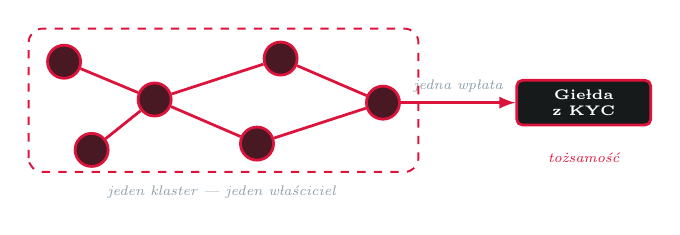
\begin{tikzpicture}[
        every node/.style={font=\tiny\bfseries, align=center},
        adr/.style={
          circle, draw=stplred, line width=1pt,
          fill=stplred!25!stplcard, text=stplwhite,
          minimum size=0.42cm, inner sep=0pt,
        },
        kyc/.style={
          draw=stplred, line width=1pt,
          fill=stplcard, text=stplwhite,
          rounded corners=2pt,
          minimum width=1.7cm, minimum height=0.55cm,
        },
        ep/.style={draw=stplred, line width=1pt},
        lbl/.style={font=\tiny\itshape, text=stplmuted},
      ]
      \node[adr] (a1) at (0.0,  0.60) {};
      \node[adr] (a2) at (1.15, 0.12) {};
      \node[adr] (a3) at (0.35,-0.52) {};
      \node[adr] (a4) at (2.45,-0.44) {};
      \node[adr] (a5) at (2.75, 0.64) {};
      \node[adr] (a6) at (4.05, 0.08) {};
      \draw[ep] (a1) -- (a2);
      \draw[ep] (a2) -- (a3);
      \draw[ep] (a2) -- (a5);
      \draw[ep] (a2) -- (a4);
      \draw[ep] (a5) -- (a6);
      \draw[ep] (a4) -- (a6);
      \node[kyc] (cex) at (6.6, 0.08) {Giełda\\z KYC};
      \draw[ep, -latex] (a6) -- (cex) node[midway, above, lbl] {jedna wpłata};
      \node[lbl, align=center] at (2.0,-1.05) {jeden klaster --- jeden właściciel};
      \node[lbl, align=center, text=stplred] at (6.6,-0.62) {tożsamość};
      \draw[draw=stplred, dashed, line width=0.7pt, rounded corners=5pt]
        (-0.45,-0.80) rectangle (4.5,1.02);
    \end{tikzpicture}
  \end{center}
  \begin{alertblock}{Pseudonim to nie anonimowość}
    Nazwisko trafia do jednego wierzchołka --- krawędzie przenoszą je na cały klaster.
  \end{alertblock}
\end{frame}

\begin{frame}{Metadane}
  \begin{itemize}
    \item Portfel nie rozmawia z siecią wprost --- rozmawia z węzłem \textbf{RPC}
    \item Dostawca RPC widzi adres IP i adres portfela w jednym zapytaniu
    \item Powiązanie powstaje poza łańcuchem i nie zostawia w nim śladu
    \item Szyfrowanie kwot nie zmienia w tym miejscu niczego
  \end{itemize}
  \vspace{0.15cm}
  \begin{center}
    \begin{tikzpicture}[
        every node/.style={font=\scriptsize\bfseries, align=center},
        box/.style={
          draw=stplred, line width=1pt,
          fill=stplcard, text=stplwhite,
          rounded corners=2pt,
          minimum width=2.0cm, minimum height=0.55cm,
        },
        arr/.style={-latex, draw=stplred, line width=0.9pt},
        lbl/.style={font=\tiny\itshape, text=stplmuted},
      ]
      \node[box] (w)   at (0.0, 0) {Portfel};
      \node[box] (rpc) at (4.0, 0) {Węzeł RPC};
      \node[box] (net) at (8.6, 0) {Sieć Solana};
      \draw[arr] (w)   -- (rpc) node[midway, above, lbl] {IP + adres};
      \draw[arr] (rpc) -- (net) node[midway, above, lbl] {transakcja};
      \node[lbl, align=center, text=stplred] at (4.0,-0.75)
        {tutaj powstaje powiązanie\\IP $\leftrightarrow$ adres};
      \draw[draw=stplred, dashed, line width=0.7pt, rounded corners=4pt]
        ($(rpc.north west)+(-0.2,0.16)$) rectangle ($(rpc.south east)+(0.2,-0.16)$);
    \end{tikzpicture}
  \end{center}
  \vspace{0.15cm}
  \begin{alertblock}{Dwie warstwy}
    Poufność w rejestrze i poufność w sieci to osobne problemy.
    Drugi z nich rozwiązuje się warstwą transportową, nie kryptografią kwot.
  \end{alertblock}
\end{frame}

% ================================================================
\section{Ukrywanie danych}

\begin{frame}{Skrót}
  \begin{itemize}
    \item Blok z Lekcji 0 i adres PDA z Lekcji 5 opierały się na tym samym
    \item W obu przypadkach pracowała ta sama \textbf{funkcja skrótu (hash)}
    \item Z dowolnie długiego wejścia liczy krótki wynik stałej długości
    \item Zmiana jednego bajtu daje zupełnie inny wynik; droga powrotna nie istnieje
  \end{itemize}
  \vspace{0.2cm}
  \begin{center}
    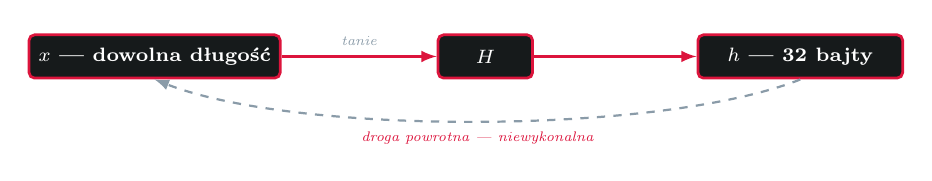
\begin{tikzpicture}[
        every node/.style={font=\scriptsize\bfseries, align=center},
        box/.style={
          draw=stplred, line width=1pt,
          fill=stplcard, text=stplwhite,
          rounded corners=2pt,
          minimum width=2.2cm, minimum height=0.55cm,
        },
        arr/.style={-latex, draw=stplred, line width=0.9pt},
        lbl/.style={font=\tiny\itshape, text=stplmuted},
      ]
      \node[box, minimum width=3.0cm] (x) at (0.0, 0) {$x$ --- dowolna długość};
      \node[box, minimum width=1.2cm] (h) at (4.2, 0) {$H$};
      \node[box, minimum width=2.6cm] (o) at (8.2, 0) {$h$ --- 32 bajty};
      \draw[arr] (x) -- (h) node[midway, above, lbl] {tanie};
      \draw[arr] (h) -- (o);
      \draw[draw=stplmuted, dashed, -latex, line width=0.8pt]
        (o.south) .. controls (6.4,-1.0) and (1.8,-1.0) .. (x.south)
        node[midway, below, lbl, text=stplred] {droga powrotna --- niewykonalna};
    \end{tikzpicture}
  \end{center}
  \vspace{0.2cm}
  \begin{block}{Funkcja skrótu}
    \[
      h = H(x)
    \]
  \end{block}
\end{frame}

\begin{frame}{Zobowiązanie}
  \begin{itemize}
    \item Typ w zakładzie trzeba podać przed meczem, nie pokazując go rywalowi
    \item Sam skrót wystarcza za zalakowaną kopertę --- wejścia nie da się podmienić
    \item Krótki zbiór możliwych wartości da się jednak przeliczyć po kolei
    \item Z losową zaślepką powstaje \textbf{zobowiązanie (commitment)}
  \end{itemize}
  \vspace{0.1cm}
  \begin{center}
    \begin{tikzpicture}[
        every node/.style={font=\scriptsize\bfseries, align=center},
        box/.style={
          draw=stplmuted, line width=1pt,
          fill=stplcard, text=stplwhite,
          rounded corners=2pt,
          minimum width=1.5cm, minimum height=0.5cm,
        },
        good/.style={box, draw=stplred},
        arr/.style={-latex, draw=stplmuted, line width=0.8pt},
        arrg/.style={-latex, draw=stplred, line width=0.9pt},
        lbl/.style={font=\tiny\itshape, text=stplmuted},
      ]
      % wiersz 1 --- sam skrót
      \node[box] (m1) at (0.0, 0.48) {$m$};
      \node[box, minimum width=1.0cm] (h1) at (2.6, 0.48) {$H$};
      \node[box, minimum width=1.8cm] (c1) at (5.4, 0.48) {$H(m)$};
      \draw[arr] (m1) -- (h1);
      \draw[arr] (h1) -- (c1);
      \node[lbl, anchor=west, text=stplred] at (6.6, 0.48)
        {kwota z zakresu $0..100$ --- 101 prób};
      % wiersz 2 --- zobowiązanie
      \node[good, minimum width=1.9cm] (m2) at (0.0,-0.62) {$m \,\|\, r$};
      \node[good, minimum width=1.0cm] (h2) at (2.6,-0.62) {$H$};
      \node[good, minimum width=1.8cm] (c2) at (5.4,-0.62) {$C$};
      \draw[arrg] (m2) -- (h2);
      \draw[arrg] (h2) -- (c2);
      \node[lbl, anchor=west, text=stplred] at (6.6,-0.62)
        {$r$ ma 256 bitów --- prób brak};
      \node[lbl, anchor=east] at (-0.85, 0.48) {bez zaślepki};
      \node[lbl, anchor=east] at (-0.95,-0.62) {z zaślepką};
    \end{tikzpicture}
  \end{center}
  \begin{block}{Zobowiązanie}
    \[
      C = H(m \,\|\, r)
    \]
    \textbf{Wiążące} --- $m$ nie da się zmienić. \textbf{Ukrywające} --- $C$ nie zdradza $m$.
  \end{block}
\end{frame}

\begin{frame}{Szyfrowanie}
  \begin{itemize}
    \item Skrzynka na listy z kłódką: wrzucić może każdy, otworzyć tylko właściciel
    \item Ta sama para kluczy działa również w drugą stronę --- to jest \textbf{szyfrowanie}
    \item Podpis tworzy klucz prywatny, a weryfikuje publiczny; szyfrogram odwrotnie
  \end{itemize}
  \vspace{-0.05cm}
  \begin{center}
    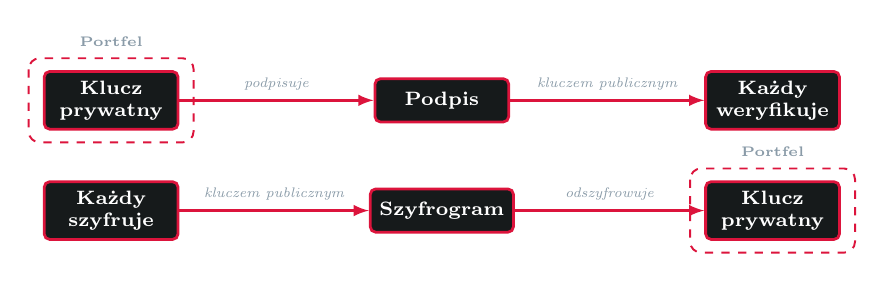
\begin{tikzpicture}[
        every node/.style={font=\scriptsize\bfseries, align=center},
        box/.style={
          draw=stplred, line width=1pt,
          fill=stplcard, text=stplwhite,
          rounded corners=2pt,
          minimum width=1.7cm, minimum height=0.55cm,
        },
        arr/.style={-latex, draw=stplred, line width=0.9pt},
        lbl/.style={font=\tiny\itshape, text=stplmuted},
      ]
      % góra: podpis --- kierunek znany z Lekcji 7
      \node[box] (sk1) at (0,    0.6) {Klucz\\prywatny};
      \node[box] (sig) at (4.2,  0.6) {Podpis};
      \node[box] (any) at (8.4,  0.6) {Każdy\\weryfikuje};
      \draw[arr] (sk1) -- (sig) node[midway, above, lbl] {podpisuje};
      \draw[arr] (sig) -- (any) node[midway, above, lbl] {kluczem publicznym};
      % dół: szyfrowanie --- ten sam rysunek odbity
      \node[box] (any2) at (0,   -0.8) {Każdy\\szyfruje};
      \node[box] (ct)   at (4.2, -0.8) {Szyfrogram};
      \node[box] (sk2)  at (8.4, -0.8) {Klucz\\prywatny};
      \draw[arr] (any2) -- (ct)  node[midway, above, lbl] {kluczem publicznym};
      \draw[arr] (ct)   -- (sk2) node[midway, above, lbl] {odszyfrowuje};
      % motyw portfela z Lekcji 7
      \foreach \n in {sk1, sk2} {
        \draw[draw=stplred, dashed, line width=0.7pt, rounded corners=4pt]
          ($(\n.north west)+(-0.18,0.15)$) rectangle ($(\n.south east)+(0.18,-0.15)$);
        \node[font=\tiny\bfseries, text=stplmuted] at ($(\n.north)+(0,0.36)$) {Portfel};
      }
    \end{tikzpicture}
  \end{center}
  \vspace{-0.3cm}
  \begin{block}{Dwa kierunki jednej pary kluczy}
    \[
      \sigma = \mathrm{Sign}(sk, m) \qquad c = \mathrm{Enc}(pk, m)
    \]
  \end{block}
\end{frame}

\begin{frame}{Homomorfizm}
  \begin{itemize}
    \item Sieć musi zaktualizować saldo, nie znając ani salda, ani kwoty przelewu
    \item Dwie zaklejone koperty z banknotami włożone do jednej --- w środku suma
    \item Niektóre szyfry pozwalają dodać szyfrogramy bez odszyfrowania
    \item \textbf{ElGamal} na krzywej eliptycznej jest homomorficzny addytywnie
  \end{itemize}
  \vspace{0.1cm}
  \begin{center}
    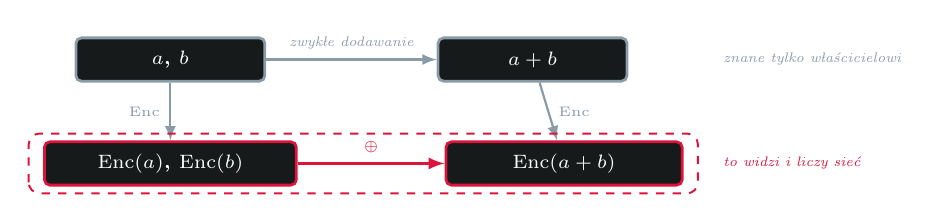
\begin{tikzpicture}[
        every node/.style={font=\scriptsize\bfseries, align=center},
        box/.style={
          draw=stplmuted, line width=1pt,
          fill=stplcard, text=stplwhite,
          rounded corners=2pt,
          minimum width=2.4cm, minimum height=0.55cm,
        },
        cbox/.style={box, draw=stplred},
        arr/.style={-latex, draw=stplmuted, line width=0.8pt},
        arrg/.style={-latex, draw=stplred, line width=1pt},
        lbl/.style={font=\tiny\itshape, text=stplmuted},
      ]
      % wiersz jawny
      \node[box]  (ab)  at (0.0, 0.70) {$a$, $b$};
      \node[box]  (s)   at (4.6, 0.70) {$a+b$};
      \draw[arr] (ab) -- (s) node[midway, above, lbl] {zwykłe dodawanie};
      % wiersz szyfrogramów
      \node[cbox, minimum width=3.2cm] (ea) at (0.0,-0.62) {$\mathrm{Enc}(a)$, $\mathrm{Enc}(b)$};
      \node[cbox, minimum width=3.0cm] (es) at (5.0,-0.62) {$\mathrm{Enc}(a+b)$};
      \draw[arrg] (ea) -- (es) node[midway, above, lbl, text=stplred] {$\oplus$};
      % strzałki pionowe
      \draw[arr] (ab) -- (ea) node[midway, left, lbl] {$\mathrm{Enc}$};
      \draw[arr] (s)  -- (es) node[midway, right, lbl] {$\mathrm{Enc}$};
      % adnotacje warstw
      \node[lbl, anchor=west] at (6.9, 0.70) {znane tylko właścicielowi};
      \node[lbl, anchor=west, text=stplred] at (6.9,-0.62) {to widzi i liczy sieć};
      \draw[draw=stplred, dashed, line width=0.7pt, rounded corners=4pt]
        (-1.8,-1.00) rectangle (6.7,-0.24);
    \end{tikzpicture}
  \end{center}
  \begin{block}{Homomorfizm addytywny}
    \[
      \mathrm{Enc}(a) \oplus \mathrm{Enc}(b) = \mathrm{Enc}(a+b)
    \]
  \end{block}
\end{frame}

\begin{frame}{Przepełnienie}
  \begin{itemize}
    \item Sieć dodaje szyfrogramy, nie wiedząc, jakie liczby dodaje
    \item Kwota jest liczbą modulo $2^{64}$ --- odejmowanie to też dodawanie
    \item Przelew ,,minus tysiąc'' zwiększyłby saldo nadawcy i stworzył tokeny
    \item \textbf{Dowód zakresu (range proof)} potwierdza, że kwota mieści się w przedziale
  \end{itemize}
  \vspace{0.1cm}
  \begin{center}
    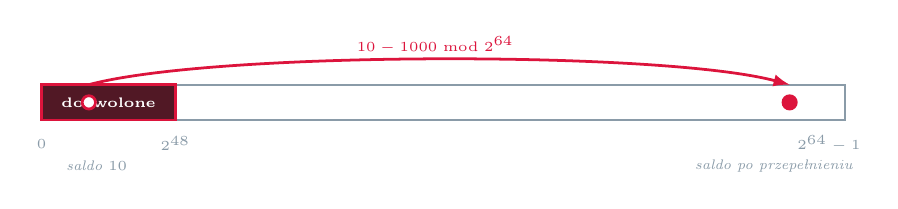
\begin{tikzpicture}[x=1cm, y=1cm,
        lbl/.style={font=\tiny\itshape, text=stplmuted},
      ]
      \draw[draw=stplmuted, line width=0.7pt] (0,0) rectangle (10.2,0.45);
      \filldraw[fill=stplred!30!stplcard, draw=stplred, line width=1pt]
        (0,0) rectangle (1.7,0.45);
      \node[font=\tiny\bfseries, text=stplwhite] at (0.85,0.225) {dozwolone};
      \node[lbl] at (0.0,-0.3)  {$0$};
      \node[lbl] at (1.7,-0.3)  {$2^{48}$};
      \node[lbl] at (10.0,-0.3) {$2^{64}-1$};
      \filldraw[fill=stplwhite, draw=stplred, line width=1pt] (0.6,0.225) circle (2.4pt);
      \filldraw[fill=stplred, draw=stplred, line width=1pt] (9.5,0.225) circle (2.4pt);
      \draw[-latex, draw=stplred, line width=1pt]
        (0.6,0.45) .. controls (2.2,0.88) and (7.9,0.88) .. (9.5,0.45);
      \node[font=\tiny\bfseries, text=stplred] at (5.0,0.95)
        {$10 - 1000 \bmod 2^{64}$};
      \node[lbl, align=center] at (9.3,-0.58) {saldo po przepełnieniu};
      \node[lbl, align=center] at (0.7,-0.58) {saldo $10$};
    \end{tikzpicture}
  \end{center}
  \vspace{0.05cm}
  \begin{alertblock}{Po co dowód zakresu}
    Homomorfizm nie chroni przed przepełnieniem --- granicę kwoty trzeba wymusić dowodem.
  \end{alertblock}
\end{frame}

% ================================================================
\section{Dowody bez ujawniania}

\begin{frame}{Dowód}
  \begin{itemize}
    \item Ochrona przy wejściu musi wiedzieć tylko jedno: czy osoba jest pełnoletnia
    \item Dowód osobisty odpowiada, ujawniając przy okazji adres i datę urodzenia
    \item Potrzebna jest sama odpowiedź --- z gwarancją, że nie została zmyślona
    \item \textbf{Zero-Knowledge Proof (ZKP)} --- dowód zdania bez ujawnienia danych
  \end{itemize}
  \vspace{0.15cm}
  \begin{block}{Trzy własności dowodu}
    \textbf{Zupełność} --- prawdę zawsze da się udowodnić.
    \textbf{Poprawność} --- fałszu nie da się.
    \textbf{Wiedza zerowa} --- weryfikator nie poznaje niczego poza odpowiedzią.
  \end{block}
  \vspace{0.1cm}
  \begin{center}
    \textcolor{stplmuted}{\small To jest trudne --- zatrzymaj film i wróć do tego slajdu}
  \end{center}
\end{frame}

% Slajd porównawczy --- statyczny (§4.5a). Bloki na takiej klatce byłyby
% niewidoczne (własny \pause), więc podpisy idą jako \item<1->.
\begin{frame}<1>{Systemy dowodowe}
  \vspace{0.2cm}
  \begin{center}
    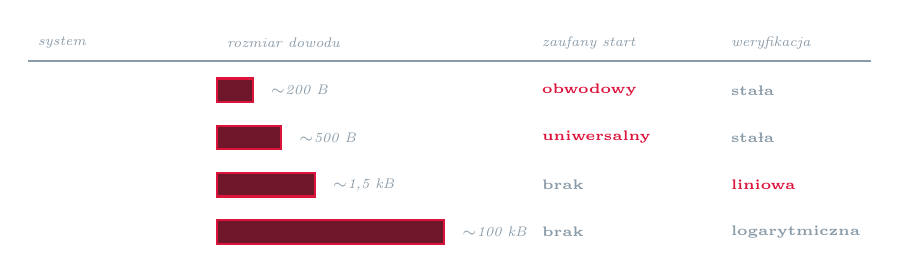
\begin{tikzpicture}[x=1cm, y=1cm,
        every node/.style={font=\tiny\bfseries, text=stplwhite},
        lbl/.style={font=\tiny\itshape, text=stplmuted},
        bar/.style={fill=stplred!45!stplcard, draw=stplred, line width=0.8pt},
      ]
      % nagłówki kolumn
      \node[lbl, anchor=west] at (0.0, 0.95) {system};
      \node[lbl, anchor=west] at (2.4, 0.95) {rozmiar dowodu};
      \node[lbl, anchor=west] at (6.4, 0.95) {zaufany start};
      \node[lbl, anchor=west] at (8.8, 0.95) {weryfikacja};
      \draw[draw=stplmuted, line width=0.5pt] (0,0.72) -- (10.7,0.72);

      % Groth16
      \node[anchor=west] at (0.0, 0.35) {Groth16};
      \filldraw[bar] (2.4,0.20) rectangle (2.85,0.50);
      \node[lbl, anchor=west] at (2.95,0.35) {$\sim$200 B};
      \node[anchor=west, text=stplred]   at (6.4,0.35) {obwodowy};
      \node[anchor=west, text=stplmuted] at (8.8,0.35) {stała};

      % PLONK
      \node[anchor=west] at (0.0,-0.25) {PLONK};
      \filldraw[bar] (2.4,-0.40) rectangle (3.21,-0.10);
      \node[lbl, anchor=west] at (3.31,-0.25) {$\sim$500 B};
      \node[anchor=west, text=stplred]   at (6.4,-0.25) {uniwersalny};
      \node[anchor=west, text=stplmuted] at (8.8,-0.25) {stała};

      % Bulletproofs
      \node[anchor=west] at (0.0,-0.85) {Bulletproofs};
      \filldraw[bar] (2.4,-1.00) rectangle (3.64,-0.70);
      \node[lbl, anchor=west] at (3.74,-0.85) {$\sim$1,5 kB};
      \node[anchor=west, text=stplmuted] at (6.4,-0.85) {brak};
      \node[anchor=west, text=stplred]   at (8.8,-0.85) {liniowa};

      % STARK
      \node[anchor=west] at (0.0,-1.45) {STARK};
      \filldraw[bar] (2.4,-1.60) rectangle (5.28,-1.30);
      \node[lbl, anchor=west] at (5.38,-1.45) {$\sim$100 kB};
      \node[anchor=west, text=stplmuted] at (6.4,-1.45) {brak};
      \node[anchor=west, text=stplmuted] at (8.8,-1.45) {logarytmiczna};
    \end{tikzpicture}
  \end{center}
  \vspace{0.25cm}
  \begin{itemize}
    % Klatka statyczna renderuje wyłącznie overlay 1 --- stąd jawne <1->.
    \item<1-> Krótki dowód kupuje się \textbf{zaufanym startem}; jego brak płaci się rozmiarem
    \item<1-> Zaufany start to jednorazowa ceremonia --- jej uczestnicy muszą usunąć sekret
    \item<1-> STARK opiera się wyłącznie na skrótach, więc przetrwa komputer kwantowy
  \end{itemize}
\end{frame}

\begin{frame}{Drzewo Merkle}
  \begin{itemize}
    \item Zobowiązań są miliony --- sprawdzanie ich po kolei nie ma prawa się skalować
    \item Skróty łączy się parami jak w drabince turniejowej, aż zostaje jeden \textbf{korzeń}
    \item Zmiana dowolnego liścia zmienia korzeń --- jedna wartość na cały zbiór
    \item Przynależność dowodzi się \textbf{ścieżką} skrótów, nie całym zbiorem
  \end{itemize}
  \vspace{-0.1cm}
  \begin{center}
    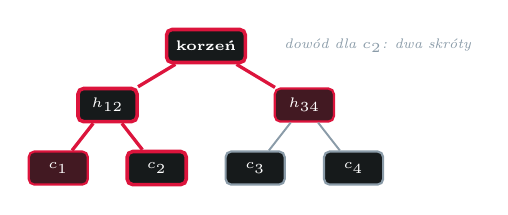
\begin{tikzpicture}[
        every node/.style={font=\tiny\bfseries},
        leaf/.style={
          draw=stplmuted, line width=0.8pt,
          fill=stplcard, text=stplwhite,
          rounded corners=2pt,
          minimum width=0.75cm, minimum height=0.42cm,
        },
        onpath/.style={leaf, draw=stplred, line width=1.3pt},
        sib/.style={leaf, draw=stplred, fill=stplred!22!stplcard},
        e/.style={draw=stplmuted, line width=0.7pt},
        ep/.style={draw=stplred, line width=1.2pt},
        lbl/.style={font=\tiny\itshape, text=stplmuted},
      ]
      \node[sib]     (c1) at (0,    0)   {$c_1$};
      \node[onpath]  (c2) at (1.25, 0)   {$c_2$};
      \node[leaf]    (c3) at (2.5,  0)   {$c_3$};
      \node[leaf]    (c4) at (3.75, 0)   {$c_4$};
      \node[onpath]  (h12) at (0.625, 0.8) {$h_{12}$};
      \node[sib]     (h34) at (3.125, 0.8) {$h_{34}$};
      \node[onpath, minimum width=1.0cm] (root) at (1.875, 1.55) {korzeń};
      \draw[ep] (c1) -- (h12);
      \draw[ep] (c2) -- (h12);
      \draw[e]  (c3) -- (h34);
      \draw[e]  (c4) -- (h34);
      \draw[ep] (h12) -- (root);
      \draw[ep] (h34) -- (root);
      \node[lbl, right=0.35cm of root] {dowód dla $c_2$: dwa skróty};
    \end{tikzpicture}
  \end{center}
  \vspace{-0.2cm}
  \begin{block}{Koszt dowodu}
    \[
      \log_2 n
    \]
    Dla miliona liści --- dwadzieścia skrótów.
  \end{block}
\end{frame}

\begin{frame}{Nullifier}
  \begin{itemize}
    \item Dowód przynależności nie wskazuje, który liść został właśnie wydany
    \item Bez dodatkowego znacznika ten sam liść dałoby się wydać wielokrotnie
    \item Wypłata publikuje \textbf{nullifier} --- wartość wyprowadzoną z sekretu noty
    \item Sieć odrzuca powtórzony nullifier, nie wiedząc, do której noty należy
  \end{itemize}
  \vspace{0.1cm}
  \begin{center}
    \begin{tikzpicture}[
        every node/.style={font=\scriptsize\bfseries, align=center},
        box/.style={
          draw=stplred, line width=1pt,
          fill=stplcard, text=stplwhite,
          rounded corners=2pt,
          minimum width=2.2cm, minimum height=0.6cm,
        },
        arr/.style={-latex, draw=stplred, line width=0.9pt},
        lbl/.style={font=\tiny\itshape, text=stplmuted},
      ]
      \node[box, minimum width=1.9cm] (note) at (0.0, 0.0) {Nota\\sekret $s$};
      \node[box, minimum width=2.6cm] (tree) at (4.2, 0.78) {Drzewo\\zobowiązań};
      \node[box, minimum width=2.6cm] (nul)  at (4.2,-0.78) {Zbiór\\nullifierów};
      \draw[arr] (note) -- (tree) node[midway, above, lbl] {$C = H(s \,\|\, v)$};
      \draw[arr] (note) -- (nul)  node[midway, below, lbl] {$N = H(s)$};
      \node[lbl, anchor=west, align=left] at (5.8, 0.78)
        {wpłata --- rośnie zbiór\\anonimowości};
      \node[lbl, anchor=west, align=left, text=stplred] at (5.8,-0.78)
        {wypłata --- $N$ już był,\\transakcja odrzucona};
      \node[lbl, align=center] at (0.0,-0.98) {$C$ i $N$ nie dają się\\powiązać bez $s$};
    \end{tikzpicture}
  \end{center}
  \begin{block}{Podwójne wydanie}
    Nullifier jest deterministyczny dla właściciela noty i losowy dla obserwatora.
  \end{block}
\end{frame}

\begin{frame}{Zbiór anonimowości}
  \begin{itemize}
    \item Urna wyborcza: karta wchodzi z tożsamością, wychodzi bez niej
    \item Obserwator wie tylko, że wypłacający jest jednym z $n$ uczestników
    \item Każde dodatkowe kryterium zawęża ten zbiór, nie łamiąc szyfru
    \item Podpis pierścieniowy i adres jednorazowy realizują ten sam pomysł inaczej
  \end{itemize}
  \vspace{0.15cm}
  \begin{center}
    \begin{tikzpicture}[x=1cm, y=1cm,
        every node/.style={font=\tiny\bfseries, text=stplwhite, align=center},
        b/.style={
          draw=stplred, line width=0.8pt,
          rounded corners=2pt, minimum height=0.4cm,
        },
        lbl/.style={font=\tiny\itshape, text=stplmuted},
      ]
      \node[b, minimum width=5.2cm, fill=stplred!20!stplcard] at (0, 0.00) {1000 wpłat w puli};
      \node[b, minimum width=3.4cm, fill=stplred!35!stplcard] at (0,-0.55) {40};
      \node[b, minimum width=1.9cm, fill=stplred!55!stplcard] at (0,-1.10) {6};
      \node[b, minimum width=0.8cm, fill=stplred]             at (0,-1.65) {1};
      \node[lbl, anchor=west] at (3.0,-0.275) {ta sama, nietypowa kwota};
      \node[lbl, anchor=west] at (3.0,-0.825) {wypłata w ciągu godziny};
      \node[lbl, anchor=west, text=stplred] at (3.0,-1.375) {znany adres odbiorcy};
    \end{tikzpicture}
  \end{center}
  \vspace{0.05cm}
  \begin{alertblock}{Anonimowość to statystyka}
    Siła ochrony zależy od liczby uczestników, nie od siły szyfru.
  \end{alertblock}
\end{frame}

% ================================================================
\section{Ekosystem}

\begin{frame}{Zcash}
  \begin{itemize}
    \item Pierwsza sieć, w której pula ekranowana zadziałała na dużą skalę
    \item Adres przejrzysty działa jak na Bitcoinie; ekranowany ukrywa strony i kwotę
    \item \textbf{Viewing key} udostępnia historię wybranej osobie --- na przykład audytorowi
    \item Od aktualizacji NU5 dowody liczy \textbf{Halo 2} --- bez ceremonii zaufanego startu
  \end{itemize}
  \vspace{0.1cm}
  \begin{exampleblock}{Komplet w jednym miejscu}
    Zobowiązanie, drzewo Merkle, nullifier i dowód ZK ---
    Zcash to cała poprzednia sekcja złożona w jeden produkt.
  \end{exampleblock}
  \vspace{-0.1cm}
  \begin{flushright}
    \textcolor{stplmuted}{\tiny z.cash · 2026}
  \end{flushright}
\end{frame}

\begin{frame}{Aleo, Mina}
  \begin{itemize}
    \item \textbf{Aleo} --- prywatność jest domyślna: pole bez adnotacji jest prywatne
    \item Program wykonuje się poza łańcuchem, a sieć weryfikuje sam dowód
    \item Stan mieszka w \textbf{rekordach} --- model bliższy UTXO niż kontu z Lekcji 5
    \item \textbf{Mina} --- dowód rekurencyjny, czyli dowód potwierdzający poprzedni dowód
    \item Cały łańcuch da się zweryfikować z około \textbf{22 kB} danych
  \end{itemize}
  \vspace{0.1cm}
  \begin{block}{Dwie różne stawki}
    Aleo kupuje za dowody poufność obliczeń.
    Mina kupuje za nie stały rozmiar łańcucha.
  \end{block}
  \vspace{-0.1cm}
  \begin{flushright}
    \textcolor{stplmuted}{\tiny aleo.org · minaprotocol.com · 2026}
  \end{flushright}
\end{frame}

\begin{frame}{Noir, zkVM}
  \begin{itemize}
    \item Obwód dowodowy pisany ręcznie to praca dla kryptografa --- i to była bariera
    \item \textbf{Noir} --- język o składni bliskiej Rustowi, kompilowany do obwodu
    \item Backend dowodowy jest wymienny --- ten sam program, różne systemy
    \item \textbf{zkVM} dowodzi wykonania zwykłego programu na maszynie RISC-V
    \item \textbf{RISC Zero} i \textbf{SP1} --- na wejściu program w Ruście, na wyjściu dowód
  \end{itemize}
  \vspace{0.1cm}
  \begin{center}
    
\begin{tikzpicture}[
        every node/.style={font=\scriptsize\bfseries, align=center},
        box/.style={
          draw=stplred, line width=1pt,
          fill=stplcard, text=stplwhite,
          rounded corners=2pt,
          minimum width=1.9cm, minimum height=0.6cm,
        },
        arr/.style={-latex, draw=stplred, line width=0.9pt},
        lbl/.style={font=\tiny\itshape, text=stplmuted},
      ]
      \node[box] (rs)  at (0.0, 0) {Program\\w Ruście};
      \node[box] (ci)  at (3.0, 0) {Obwód};
      \node[box] (pf)  at (6.0, 0) {Dowód};
      \node[box, minimum width=2.1cm] (vf) at (9.1, 0) {Weryfikator\\w łańcuchu};
      \draw[arr] (rs) -- (ci) node[midway, above, lbl] {kompilacja};
      \draw[arr] (ci) -- (pf) node[midway, above, lbl] {backend};
      \draw[arr] (pf) -- (vf) node[midway, above, lbl] {kilka kB};
      \draw[draw=stplred, dashed, line width=0.7pt, rounded corners=4pt]
        (4.05,-0.42) rectangle (4.95,0.42);
      \node[lbl, align=center] at (4.5,-0.72) {wymienny};
    \end{tikzpicture}
  \end{center}
  \begin{exampleblock}{Co to zmienia}
    Dowód przestaje być projektem kryptograficznym, a staje się biblioteką.
  \end{exampleblock}
  \vspace{-0.1cm}
  \begin{flushright}
    \textcolor{stplmuted}{\tiny noir-lang.org · risczero.com · 2026}
  \end{flushright}
\end{frame}

% ================================================================
\section{Poufność na Solanie}

\begin{frame}{Token-2022}
  \begin{itemize}
    \item \textbf{Token-2022} to nowszy program tokenowy Solany, z rozszerzeniami
    \item Rozszerzenie \textbf{confidential transfers} szyfruje kwoty przelewów i salda kont
    \item Sieć nadal sprawdza: środków starczyło i nic nie powstało z niczego
    \item Sprawdza to dowodem, nie odczytem --- mechanizmem z poprzedniej sekcji
  \end{itemize}
  \vspace{0.25cm}
  \begin{alertblock}{Co nie jest ukryte}
    Adresy nadawcy i odbiorcy pozostają jawne.
    Solana ukrywa kwoty, nie tożsamości.
  \end{alertblock}
\end{frame}

\begin{frame}{Trzy salda}
  \begin{itemize}
    \item \textbf{Public} --- zwykłe, jawne saldo SPL
    \item \textbf{Pending} --- zaszyfrowane wpłaty przychodzące, jeszcze niezaksięgowane
    \item \textbf{Available} --- zaszyfrowane saldo gotowe do wydania
    \item Przeniesienie z \emph{pending} do \emph{available} wykonuje właściciel osobną instrukcją
  \end{itemize}
  \vspace{0.1cm}
  \begin{center}
    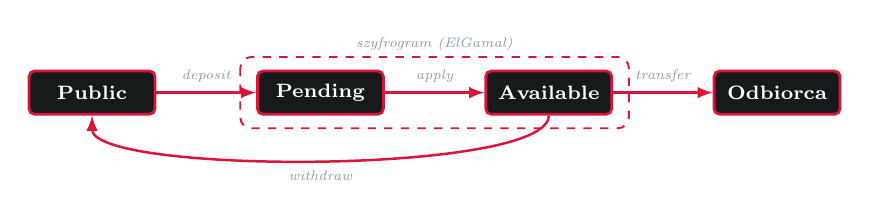
\begin{tikzpicture}[
        every node/.style={font=\scriptsize\bfseries, align=center},
        box/.style={
          draw=stplred, line width=1pt,
          fill=stplcard, text=stplwhite,
          rounded corners=2pt,
          minimum width=1.6cm, minimum height=0.55cm,
        },
        arr/.style={-latex, draw=stplred, line width=0.9pt},
        lbl/.style={font=\tiny\itshape, text=stplmuted},
      ]
      \node[box] (pub) at (0,   0) {Public};
      \node[box] (pen) at (2.9, 0) {Pending};
      \node[box] (ava) at (5.8, 0) {Available};
      \node[box] (rec) at (8.7, 0) {Odbiorca};
      \draw[arr] (pub) -- (pen) node[midway, above, lbl] {deposit};
      \draw[arr] (pen) -- (ava) node[midway, above, lbl] {apply};
      \draw[arr] (ava) -- (rec) node[midway, above, lbl] {transfer};
      \draw[arr] (ava.south) .. controls +(0,-0.75) and +(0,-0.75) .. (pub.south)
        node[midway, below, lbl] {withdraw};
      \draw[draw=stplred, dashed, line width=0.7pt, rounded corners=4pt]
        ($(pen.north west)+(-0.2,0.16)$) rectangle ($(ava.south east)+(0.2,-0.16)$);
      \node[lbl] at (4.35, 0.62) {szyfrogram (ElGamal)};
    \end{tikzpicture}
  \end{center}
  \begin{block}{Dwa klucze z jednej pary}
    \textbf{ElGamal} szyfruje kwoty przelewów, \textbf{AES} odszyfrowuje własne saldo.
  \end{block}
\end{frame}

\begin{frame}{Trzy dowody}
  \begin{itemize}
    \item Sieć musi sprawdzić trzy rzeczy, nie poznając żadnej kwoty
    \item \textbf{Equality} --- nowe saldo nadawcy zgadza się z odjętą kwotą
    \item \textbf{Ciphertext validity} --- odbiorca zdoła odszyfrować to, co dostał
    \item \textbf{Range} --- kwota i saldo mieszczą się w dozwolonym przedziale
  \end{itemize}
  \vspace{0.1cm}
  \begin{center}
    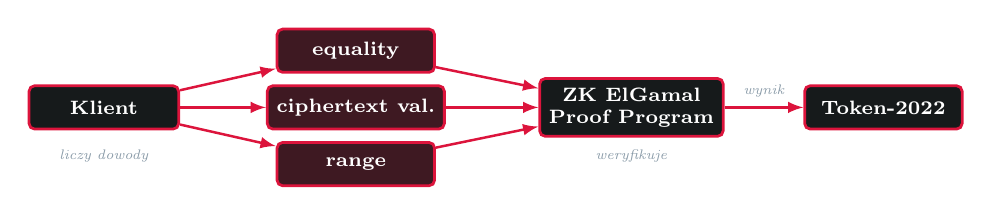
\begin{tikzpicture}[
        every node/.style={font=\scriptsize\bfseries, align=center},
        box/.style={
          draw=stplred, line width=1pt,
          fill=stplcard, text=stplwhite,
          rounded corners=2pt,
          minimum width=1.9cm, minimum height=0.55cm,
        },
        pbox/.style={box, fill=stplred!20!stplcard, minimum width=2.0cm},
        arr/.style={-latex, draw=stplred, line width=0.9pt},
        lbl/.style={font=\tiny\itshape, text=stplmuted},
      ]
      \node[box] (cli) at (0.0, 0.0) {Klient};
      \node[pbox] (eq) at (3.2, 0.72) {equality};
      \node[pbox] (cv) at (3.2, 0.00) {ciphertext val.};
      \node[pbox] (rg) at (3.2,-0.72) {range};
      \node[box, minimum width=2.3cm, align=center] (zk) at (6.7, 0.0)
        {ZK ElGamal\\Proof Program};
      \node[box, minimum width=2.0cm] (t22) at (9.9, 0.0) {Token-2022};
      \draw[arr] (cli) -- (eq);
      \draw[arr] (cli) -- (cv);
      \draw[arr] (cli) -- (rg);
      \draw[arr] (eq) -- (zk);
      \draw[arr] (cv) -- (zk);
      \draw[arr] (rg) -- (zk);
      \draw[arr] (zk) -- (t22) node[midway, above, lbl] {wynik};
      \node[lbl, align=center] at (0.0,-0.62) {liczy dowody};
      \node[lbl, align=center] at (6.7,-0.62) {weryfikuje};
    \end{tikzpicture}
  \end{center}
  \begin{block}{Podział pracy}
    Klient liczy dowody, osobny program systemowy je weryfikuje, Token-2022 czyta wynik.
  \end{block}
\end{frame}

\begin{frame}{Siedem transakcji}
  \begin{itemize}
    \item Transakcja Solany mieści \textbf{1232 bajty} --- trzy dowody się w niej nie mieszczą
    \item Każdy dowód trafia najpierw do osobnego \textbf{konta kontekstu}
    \item Właściwy transfer czyta trzy konta i wykonuje operację na szyfrogramach
    \item Konta trzeba potem zamknąć, żeby odzyskać zapłacony rent
  \end{itemize}
  \vspace{0.1cm}
  \begin{center}
    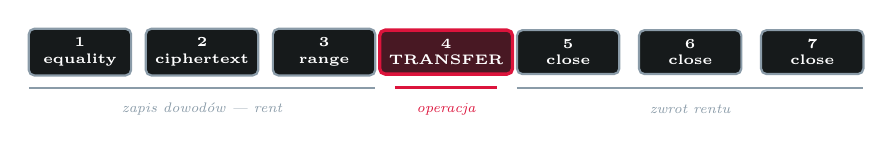
\begin{tikzpicture}[x=1cm, y=1cm,
        every node/.style={font=\tiny\bfseries, text=stplwhite, align=center},
        b/.style={
          draw=stplmuted, line width=0.8pt,
          fill=stplcard, rounded corners=2pt,
          minimum width=1.3cm, minimum height=0.55cm,
        },
        hot/.style={b, draw=stplred, line width=1.2pt, fill=stplred!25!stplcard},
        lbl/.style={font=\tiny\itshape, text=stplmuted},
      ]
      \node[b]   at (0.00,0) {1\\equality};
      \node[b]   at (1.55,0) {2\\ciphertext};
      \node[b]   at (3.10,0) {3\\range};
      \node[hot] at (4.65,0) {4\\TRANSFER};
      \node[b]   at (6.20,0) {5\\close};
      \node[b]   at (7.75,0) {6\\close};
      \node[b]   at (9.30,0) {7\\close};
      \draw[draw=stplmuted, line width=0.7pt] (-0.65,-0.45) -- (3.75,-0.45);
      \draw[draw=stplred,   line width=0.9pt] (4.00,-0.45) -- (5.30,-0.45);
      \draw[draw=stplmuted, line width=0.7pt] (5.55,-0.45) -- (9.95,-0.45);
      \node[lbl] at (1.55,-0.72) {zapis dowodów --- rent};
      \node[lbl, text=stplred] at (4.65,-0.72) {operacja};
      \node[lbl] at (7.75,-0.72) {zwrot rentu};
    \end{tikzpicture}
  \end{center}
  \vspace{0.1cm}
  \begin{alertblock}{Cena poufności}
    Wąskim gardłem jest limit rozmiaru transakcji, nie kryptografia.
    Jeden przelew to siedem podpisów i siedem opłat.
  \end{alertblock}
  \vspace{-0.15cm}
  \begin{flushright}
    \textcolor{stplmuted}{\tiny spl.solana.com/token-2022 · 2026}
  \end{flushright}
\end{frame}

\begin{frame}{Audytor}
  \begin{itemize}
    \item Firma potrzebuje poufności wobec konkurencji, nie wobec księgowego
    \item Mint wybiera jeden z czterech trybów poufności --- od wyłączonej po wymaganą
    \item Opcjonalny \textbf{auditor} to dodatkowy klucz ElGamal zapisany w mincie
    \item Auditor odszyfrowuje kwoty przelewów --- sald nie odszyfrowuje
  \end{itemize}
  \vspace{0.1cm}
  \begin{center}
    \begin{tikzpicture}[x=1cm, y=1cm,
        lbl/.style={font=\tiny\itshape, text=stplmuted},
      ]
      \begin{scope}
        \clip[rounded corners=4pt] (0,0) rectangle (10.4,0.55);
        \shade[left color=stplmuted!30!stplcard, right color=stplred]
          (0,0) rectangle (10.4,0.55);
      \end{scope}
      \draw[rounded corners=4pt, draw=stplmuted, line width=0.4pt]
        (0,0) rectangle (10.4,0.55);
      \foreach \x in {2.6,5.2,7.8}
        \draw[draw=stpldark, line width=1pt] (\x,0) -- (\x,0.55);
      \node[font=\tiny\bfseries, text=stplwhite] at (1.3,0.275) {Disabled};
      \node[font=\tiny\bfseries, text=stplwhite] at (3.9,0.275) {Whitelisted};
      \node[font=\tiny\bfseries, text=stplwhite] at (6.5,0.275) {OptIn};
      \node[font=\tiny\bfseries, text=stplwhite] at (9.1,0.275) {Required};
      \node[lbl] at (1.3,-0.32) {poufność wyłączona};
      \node[lbl] at (3.9,-0.32) {lista dopuszczonych};
      \node[lbl] at (6.5,-0.32) {wybór właściciela};
      \node[lbl, text=stplred] at (9.1,-0.32) {wymuszona na wszystkich};
      \node[lbl] at (5.2,0.85) {tryb ustawia mint --- nie da się go zmienić po wydaniu};
    \end{tikzpicture}
  \end{center}
  \vspace{0.15cm}
  \begin{exampleblock}{Po co tryby}
    Emitent stablecoina może wymusić poufność dla wszystkich i zachować wgląd
    audytora --- zgodność bez jawnych kwot.
  \end{exampleblock}
\end{frame}

\begin{frame}{Granice}
  \begin{itemize}
    \item Rozszerzenie działa dziś na testowej sieci ZK-Edge, a nie na mainnecie
    \item Generowanie dowodów obciąża klienta, a nie sieć
    \item Klucze są deterministyczne: wyciek klucza portfela odsłania całą historię sald
    \item Kwoty są ukryte, ale sam graf przelewów pozostaje w pełni czytelny
  \end{itemize}
  \vspace{0.15cm}
  \begin{alertblock}{Stan na dziś}
    Technologia przed premierą. Warto ją rozumieć --- nie warto na niej dziś
    budować produkcji.
  \end{alertblock}
  \vspace{-0.1cm}
  \begin{flushright}
    \textcolor{stplmuted}{\tiny zk-edge.surfnet.dev · 2026}
  \end{flushright}
\end{frame}

% ================================================================
\section{Podsumowanie}

% Slajd macierzowy --- statyczny (§4.5a), podpisy jako \item<1->.
\begin{frame}<1>{Macierz prymitywów}
  \vspace{0.2cm}
  \begin{center}
    \begin{tikzpicture}[x=1cm, y=1cm,
        every node/.style={font=\tiny\bfseries, text=stplwhite},
        lbl/.style={font=\tiny\itshape, text=stplmuted},
      ]
      % nagłówki
      \node[lbl, anchor=west] at (0.0, 0.95) {rozwiązanie};
      \node[lbl] at (3.9, 0.95) {kwota};
      \node[lbl] at (5.3, 0.95) {nadawca};
      \node[lbl] at (6.7, 0.95) {odbiorca};
      \node[lbl] at (8.1, 0.95) {graf};
      \node[lbl, anchor=west] at (8.8, 0.95) {koszt};
      \draw[draw=stplmuted, line width=0.5pt] (0,0.72) -- (10.9,0.72);

      % Pula ekranowana --- wszystko ukryte
      \node[anchor=west] at (0.0, 0.35) {Pula ekranowana};
      \foreach \x in {3.9,5.3,6.7,8.1}
        \filldraw[fill=stplred, draw=stplred, line width=0.8pt] (\x,0.35) circle (3.2pt);
      \node[lbl, anchor=west] at (8.8, 0.35) {dowód przy wypłacie};

      % Token-2022 --- tylko kwota
      \node[anchor=west] at (0.0,-0.25) {Token-2022};
      \filldraw[fill=stplred, draw=stplred, line width=0.8pt] (3.9,-0.25) circle (3.2pt);
      \foreach \x in {5.3,6.7,8.1}
        \draw[draw=stplmuted, line width=0.8pt] (\x,-0.25) circle (3.2pt);
      \node[lbl, anchor=west] at (8.8,-0.25) {siedem transakcji};

      % Adres jednorazowy --- tylko odbiorca
      \node[anchor=west] at (0.0,-0.85) {Adres jednorazowy};
      \foreach \x in {3.9,5.3,8.1}
        \draw[draw=stplmuted, line width=0.8pt] (\x,-0.85) circle (3.2pt);
      \filldraw[fill=stplred, draw=stplred, line width=0.8pt] (6.7,-0.85) circle (3.2pt);
      \node[lbl, anchor=west] at (8.8,-0.85) {skanowanie wszystkich wyjść};

      % Podpis pierścieniowy --- tylko nadawca
      \node[anchor=west] at (0.0,-1.45) {Podpis pierścieniowy};
      \foreach \x in {3.9,6.7,8.1}
        \draw[draw=stplmuted, line width=0.8pt] (\x,-1.45) circle (3.2pt);
      \filldraw[fill=stplred, draw=stplred, line width=0.8pt] (5.3,-1.45) circle (3.2pt);
      \node[lbl, anchor=west] at (8.8,-1.45) {podpis rośnie z $n$};

      % legenda
      \filldraw[fill=stplred, draw=stplred, line width=0.8pt] (3.9,-2.05) circle (3.2pt);
      \node[lbl, anchor=west] at (4.1,-2.05) {ukryte};
      \draw[draw=stplmuted, line width=0.8pt] (5.6,-2.05) circle (3.2pt);
      \node[lbl, anchor=west] at (5.8,-2.05) {jawne};
    \end{tikzpicture}
  \end{center}
  \vspace{0.2cm}
  \begin{itemize}
    \item<1-> Żaden pojedynczy prymityw nie ukrywa wszystkiego za darmo
    \item<1-> Wybór zaczyna się od pytania, co konkretnie ma zostać ukryte
  \end{itemize}
\end{frame}

\begin{frame}{Podsumowanie}
  \begin{enumerate}
    \item Podpis daje autentyczność --- \textbf{poufność} trzeba dołożyć osobno
    \item \textbf{Zobowiązanie}, \textbf{drzewo Merkle} i \textbf{nullifier} tworzą pulę ekranowaną
    \item Dowód ZK kupuje się rozmiarem, zaufanym startem albo czasem weryfikacji
    \item \textbf{Homomorfizm} liczy na szyfrogramach, \textbf{dowód zakresu} pilnuje granic
    \item Token-2022 ukrywa \textbf{kwoty}, nie \textbf{tożsamości} --- za cenę siedmiu transakcji
  \end{enumerate}
  \vspace{0.2cm}
  \begin{exampleblock}{Efekt}
    Prywatność na łańcuchu nie jest przełącznikiem, tylko doborem prymitywów
    do tego, co konkretnie ma zostać ukryte.
  \end{exampleblock}
\end{frame}

% ================================================================
\begin{frame}[plain]
  \begin{center}
    \vfill
    {\Huge\bfseries\color{stplwhite} gn}
    \vfill
  \end{center}
\end{frame}

\end{document}
